\chapter[Introdución]{
  \label{chp:introduccion}
  Introdución
}
\minitoc
\newpage

Nos últimos anos, Internet converteuse nunha peza importante para os \textbf{medios de radiodifusión}, xa que permite un alcance global e o acceso baixo demanda aos contidos emitidos. Isto é especialmente interesante para as pequenas emisoras locais, a miúdo \textbf{comunitarias}, culturais e con orzamento limitado ás que comunmente se fai referencia coma \textbf{medios do terceiro sector}.

A estas últimas está orientado este proxecto. Consiste nun punto de encontro en liña para promover contidos radiofónicos e favorecer a súa redifusión por parte de distintos medios de comunicación (Emisoras, canles de podcasting...) así coma o seu consumo directo por parte dos visitantes da web. Para o seu desenvolvemento, utilizouse Django, un framework web de Python, ferramentas HTML5, JavaScript e CSS-Grid. Tamén se utilizaron ferramentas de sindicación RSS para o acceso aos contidos de terceiros.

Nesta memoria tratarase o proceso completo de desenvolvemento do proxecto desde as fases de análise e deseño até os detalles de implementación. Mencionaranse tamén as liñas de traballo que se pretenden seguir no futuro.

\section{Marco do proxecto}


A radiodifusión tradicional, entendendo esta coma a retransmisión de contidos de audio a través de ondas analóxicas, presenta a día de hoxe unha serie de limitacións. A máis importante, se cadra, é o feito de que a demanda de frecuencias é superior ao que o espectro radioeléctrico pode ofrecer. Cómpre, por iso, a existencia de unha autoridade que outorgue \textbf{licenzas de emisión} sendo, neste país, a \textit{Secretaría de Estado de Telecomunicaciones y para la Sociedad de la Información} e máis a \textit{Secretaría Xeral de Medios} da Xunta de Galicia\cite{BOE}. Isto implica a imposibilidade de emitir contidos por parte de aqueles que ou ben non poidan facer fronte á inversión que unha licenza supón ou ben non lles fose outorgada.

A medida que o acceso a Internet se fai máis cotián, a \textbf{emisión por streaming} eríxese coma solución aos problemas da radio en FM. A través deste medio, unha emisora pode emitir contidos sen necesidade de licenzas, acadando unha cobertura global. Este tipo de emisión, ademais, non require de cadeas de radio enlace, como é costume nas grandes emisoras en FM, coa inversión en infraestruturas que tal cousa implica.

Internet permite non só a emisión en directo mediante streaming, senón tamén o acceso a contidos baixo demanda co nacemento do \textbf{podcasting} a mediados da década dos 2000\cite{guardian}. A aparición de ferramentas de uso diario que permiten un acceso fácil a estes contidos está a afectar ao comportamento dos usuarios: Actualmente, un 7.5\% dos ouvintes escoitan a radio por Internet; aínda lonxe dos ouvintes de FM, porén máis do dobre dos de Onda Media\cite{EGM}.

\begin{figure}[H]
	\centering
	\includegraphics[scale=0.4,keepaspectratio=true]{./images/tabla_internet_radio.png}
  	\caption{Ouvintes de radio promedio diario do ano 2017 en España.}
	\label{fig:table_egm}
\end{figure}

\section{Motivación}

Por consecuencia da falta de regulamentación específica e a desgana das institucións públicas, os medios do  terceiro sector atopan a miúdo serias dificultades para realizar a súa actividade a través da FM. Para comprender a gravidade desta situación, cómpre recordar que se está a falar de entidades pequenas, comunitarias, sen ánimo de lucro, independentes e con finalidade maioritariamente cultural e social\cite{fesp}. O \textbf{impacto positivo na pluralidade informativa} e no desenvolvemento da sociedade civil destes medios está explicitamente recoñecido pola UNESCO\cite{unesco}. 

Se ben a emisión por streaming e o podcast se perfilan coma a alternativa nun futuro inmediato, tamén veñen acompañados de certa aura de incerteza. Hai que ter en conta que os intereses deste tipo de emisoras adoitan ser de ámbito local pois os asuntos que unha radio comunitaria ten capacidade de tratar rara vez son internacionais . 

Deste xeito, a vantaxe de globalidade que ofrece Internet acaba por non ser tal. Pola contra, a súa visibilidade si queda diluída pola numerosa oferta existente a ese nivel.


\section{Orixe do proxecto}

Produciuse un encontro informal con membros de \textbf{Cuac FM} (a radio comunitaria da Coruña) e a \textbf{URCM}(Unión de Radios Comunitarias de Madrid) onde se entrou en contacto cos usuarios finais do proxecto a realizar. 

A URCM está composta por unha serie de emisoras independentes e con programas de seu. Conta cunha páxina web onde os usuarios teñen acceso a un \textbf{directorio cos ficheiros de audio} publicados por ditas emisoras (ver figura \ref{fig:urcm})\cite{urcm}. Esta sección da web, pese a súas limitacións, leva funcionando uns anos e resultou ser moi positiva para a redifusión dos programas por distintos colectivos.


\begin{figure}[h]
	\centering
	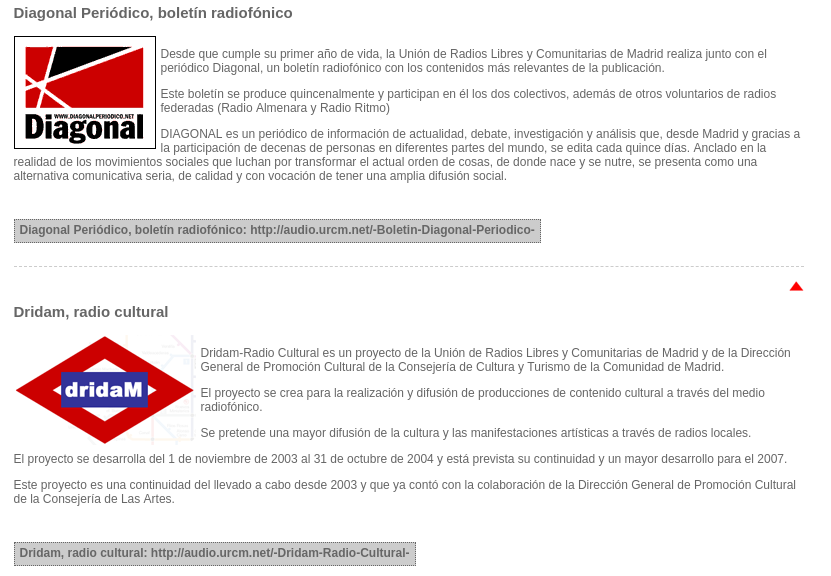
\includegraphics[scale=0.55,keepaspectratio=true]{./images/urcm.png}
	\caption{Sección de audios da web da URCM que inspira o proxecto.}
	\label{fig:urcm}
\end{figure}

Inspirados nesta idea, propúxose crear unha ferramenta semellante, pero cun conxunto de funcionalidades máis ambicioso. Esta vez para uso potencial da \textbf{ReMC} (Red de Medios Comunitarios), unha federación de medios comunitarios do Estado Español.


\section{Obxectivos}
\label{obxectivos}

Este proxecto pretende servir de axuda aos colectivos do terceiro sector da comunicación, favorecendo a colaboración entre eles e achegándolles as ferramentas necesarias para \textbf{acadar unha maior presenza na rede}.

O produto resultante consistirá nun \textbf{portal web} onde os usuarios poderán acceder a un \textbf{catálogo de programas}. O mencionado catálogo estará constituído por arquivos de son enlazados por outros usuarios que desexen compartilos desde o seu propio almacenamento.

Os obxectivos a acadar son os seguintes:

\begin{itemize}
\item Facilitar desde un portal web o acceso a ficheiros de audio mediante streaming por Internet e descarga directa desde servidores alleos ao servizo.
\item Permitir a distintos usuarios a publicación, manual ou automatizada, do seu contido no sitio web de xeito organizado por programas e categorías.
\item Ofrecer aos visitantes ferramentas de procura de contidos e a opción de subscribirse aos diferentes programas ou canais.
\item Permitir a colaboración entre usuarios na xestión de contidos publicados.
\end{itemize}



\section{Organización da memoria}

Esta memoria consta de dez capítulos, incluído este mesmo. A continuación explícase brevemente cada un deles:

\begin{itemize}
	\item \textbf{Capítulo \ref{chp:introduccion}, Introdución:} Explicación das motivacións e a orixe do proxecto. Defínense aquí, tamén os obxectivos a cumprir.
	\item \textbf{Capítulo \ref{chp:estado_da_arte}, Estado da arte:} Comparación do proxecto presentado con outros produtos software existentes na actualidade. Arguméntase por que o primeiro cumpre de xeito máis amplo e preciso cos obxectivos marcados.
	\item \textbf{Capítulo \ref{chp:tecnologia}, Tecnoloxía:} Mostra das ferramentas, bibliotecas, linguaxes e \say{frameworks} utilizados no desenvolvemento do proxecto e máis na confección desta memoria.
	\item \textbf{Capítulo \ref{chp:metodoloxia}, Metodoloxía:} Comentario das diferentes técnicas e metodoloxías para o desenvolvemento de software que se seguiron neste proxecto.
	\item \textbf{Capítulo \ref{chp:analise}, Análise:} Exposición do funcionamento ideal xeral do sistema e os requirimentos funcionais e non-funcionais que este debe cumprir.
	\item \textbf{Capítulo \ref{chp:disenho}, Deseño:} Percorrido pola arquitectura do sistema explicando a interacción entre as súas compoñentes e os patróns de deseño utilizados.
 	\item \textbf{Capítulo \ref{chp:implementacion}, Implementación:} Mostra das solucións de implementación aplicadas a certas partes do sistema especialmente complexas ou que non fosen tratadas nos capítulos anteriores.
 	\item \textbf{Capítulo \ref{chp:plan}, Planificación:} Diario de traballo que explica a recolección de historias de usuario e os avances do desenvolvemento a través do tempo. Inclúe a avaliación de custes.
 	\item \textbf{Capítulo \ref{chp:test}, Probas do sistema:} Repaso do traballo de validación realizado sobre as distintas partes do sistema.
 	\item \textbf{Capítulo \ref{chp:conclusiones}, Conclusións:}Valoración persoal do traballo, comparando o resultado final cos obxectivos previos. Inclúe unha breve reflexión sobre os coñecementos acadados e unha guía de traballos que se poderían realizar no futuro co fin de mellorar o produto desenvolvido.
	
\end{itemize}


Tamén se inclúen, a maiores, nesta memoria, tres apéndices:

\begin{itemize}
	\item \textbf{Apéndice \ref{chp:dicionario}, Dicionario de datos:} Lista das entidades do modelo de datos detallando dos seus atributos.
	\item \textbf{Apéndice \ref{chp:licenza}, Licenza:} Relación das licenzas das dependencias do proxecto e determinación das licenzas baixo as que se distribúe a aplicación creada e esta documentación.
	\item \textbf{Apéndice \ref{chp:usermanual}, Manual de usuario:} Instrucións de uso da aplicación web.
\end{itemize}

